\chapter{Projektzielsetzung}
\textbf{Projekttitel:}\\
Integriertes Demosystem für Sensor- und Displayansteuerung auf FPGA-Basis\\
\textbf{Teammitglieder:}\\
Fabian Becker, Jendrik Jürgens, Nicolas Koch, Franz Krempl, Daniel Sowada, Michael Specht\\
\textbf{Projektbeschreibung:}\\
Ziel des Projekts ist die Entwicklung und Integration eines funktionsfähigen Demosystems, das zwei getrennte Komponenten – den Sonarsensor (PMOD MAXSONAR) und das LCD-Display (PMOD CLP) – auf einer gemeinsamen FPGA-Plattform (Digilent Arty A7-100) vereint. Die Messwerte des Sensors sollen in Echtzeit auf dem Display ausgegeben werden. Dazu werden eigene IP-Cores für beide Komponenten entworfen, implementiert, getestet und in die Hardwareplattform integriert.\\\\
\textbf{Geplante Arbeitspakete und Zuständigkeiten:}
\begin{enumerate}
   \item Systemintegration bestehender Demosysteme
   \begin{itemize}
     \item Integration der Software- und Hardware-Demoprojekte zu einem Gesamtsystem (HW \& SW)
     \begin{description}
       \item[Zuständig:] Alle Teammitglieder
     \end{description}
   \end{itemize}
   \item Entwicklung Custom IP für Sensor (UART / MAXSONAR)
   \begin{itemize}
     \item Konzept (Blockdiagramm, Registermapping) auf Basis der \texttt{tut\_int} Vorlage
     \item Reduzierte Funktionalität orientiert an Xilinx UART Lite IP
     \begin{description}
       \item[Zuständig:] Fabian Becker, Nicolas Koch
     \end{description}
   \end{itemize}
   \item Entwicklung Custom IP für Display (PMOD CLP, Nibble-Mode)
   \begin{itemize}
     \item Umsetzung von Timinganforderungen in Hardware
     \item Anzeige von Daten auf LCD über FSM und spezifizierte Steuerregister
     \begin{description}
       \item[Zuständig:] Jendrik Jürgens, Michael Specht
     \end{description}
   \end{itemize}
   \item Erstellung und Test der IP-Testbenches (Core und AXI)
   \begin{itemize}
     \item Entwicklung mit Fokus auf Polling (Interrupt optional bei Zeitreserve)
     \item Simulation und Validierung des Verhaltens
     \begin{description}
       \item[Zuständig:] Alle Teammitglieder
     \end{description}
   \end{itemize}
   \item Treibersoftware
   \begin{itemize}
     \item Schreiben von Treibern für die beiden IPs unter Verwendung der SW-Templates von \texttt{tut\_int}
     \item SW-basierte Initialisierung und Datentransfer
     \begin{description}
       \item[Zuständig:] Franz Krempl, Daniel Sowada
     \end{description}
   \end{itemize}
   \item Integration in vollständiges Demosystem
   \begin{itemize}
     \item Zusammenführung aller Komponenten zu einem lauffähigen System
     \item Validierung auf der realen Hardwareplattform
     \begin{description}
       \item[Zuständig:] Alle Teammitglieder
     \end{description}
   \end{itemize}
\end{enumerate}
\textbf{Systemblockbild:}\\
\begin{figure}[h!]
  \centering
  \begin{minipage}{\textwidth}
      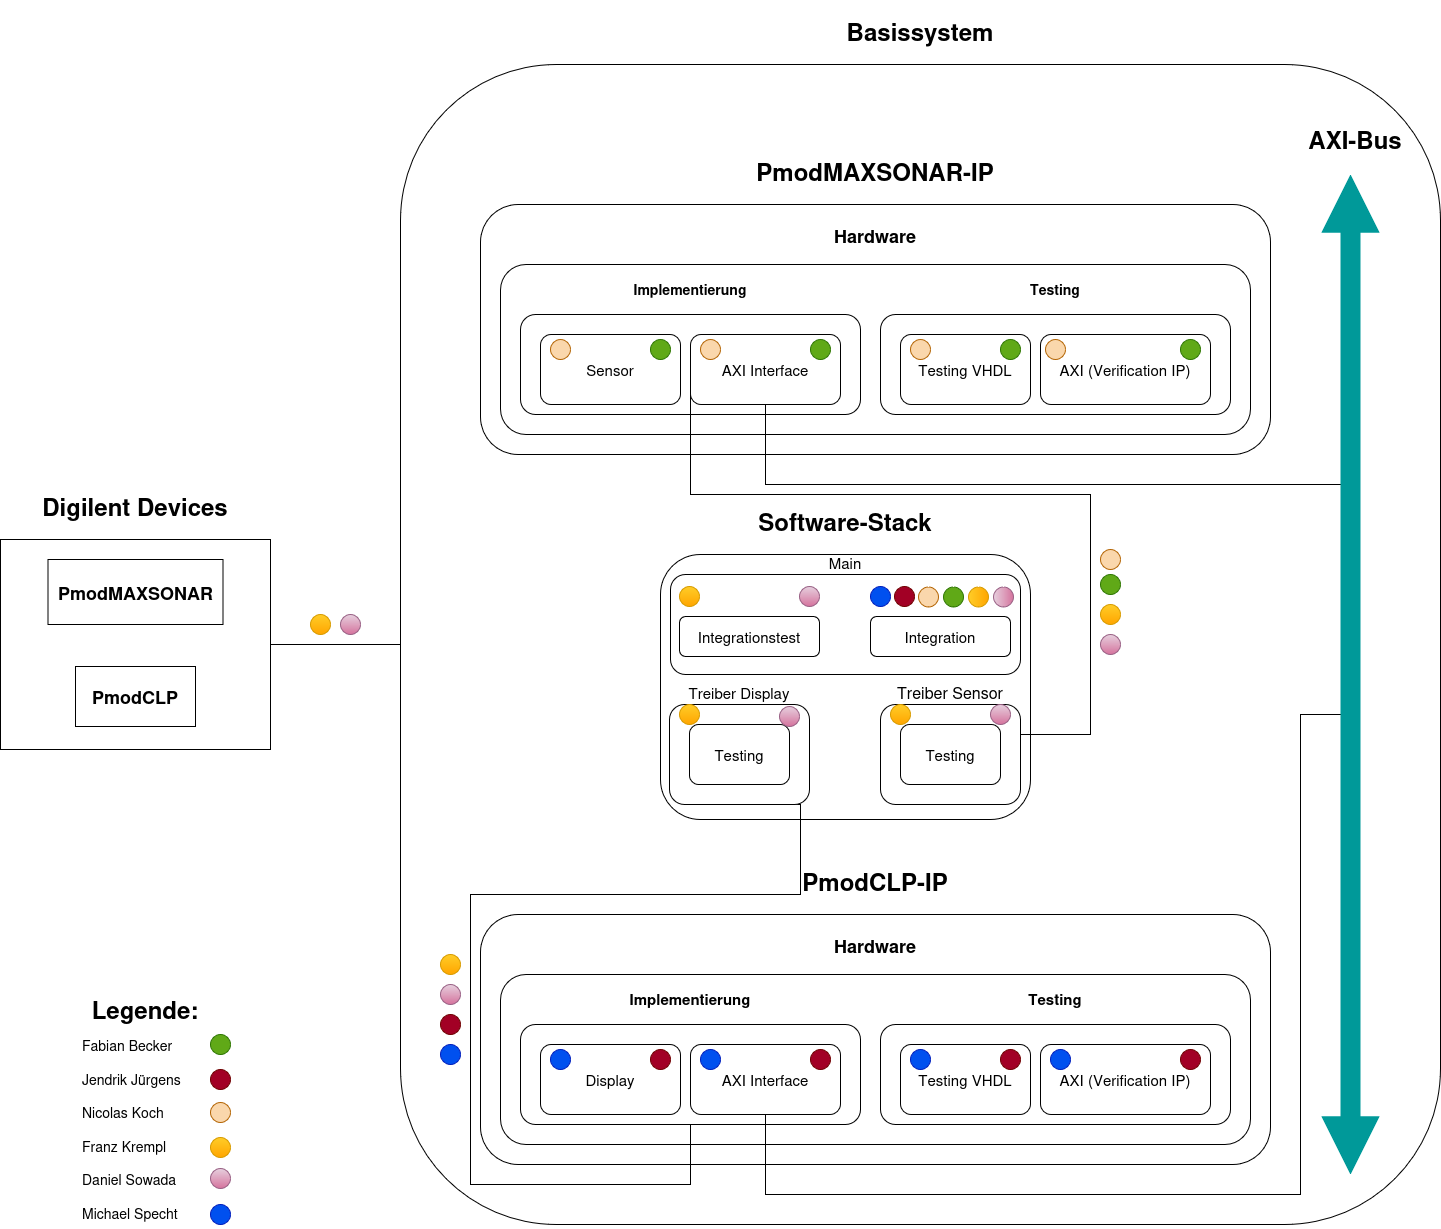
\includegraphics[width=\linewidth]{./images/system_updated_white.drawio.png} % replace with your image filename
  \end{minipage}
  \caption{Systemblockbild}
  \label{fig:system}
\end{figure}
\begin{itemize}
  \item \textbf{Exakte Timings für das Display (PmodCLP) in VHDL:}\\
  Die Ansteuerung im Nibble-Mode erfordert die präzise Umsetzung aller Timingbedingungen in einer FSM, da keine automatische Verzögerung durch die CPU gegeben ist.
\item \textbf{Entwicklung AXI4-Lite-kompatibler IP-Cores:}\\
  Für Sensor und Display werden eigenständige IPs mit klar strukturiertem Registermapping und AXI-Anbindung erstellt, basierend auf einer gemeinsamen IP-Vorlage.
\item \textbf{Zuverlässiger Datenfluss zwischen Sensor, CPU und Display:}\\
  Die Software muss synchronisiert mit den IPs arbeiten, um Sensordaten korrekt auszulesen und anzuzeigen – inklusive Fehlerbehandlung und Statusabfrage.
\item \textbf{Simulation und Verifikation:}\\
  Funktion und Schnittstellen werden über VHDL-Testbenches (Core + AXI) geprüft, um Designfehler frühzeitig zu erkennen.
\end{itemize}
\textbf{Ziel:}\\
Ein lauffähiges Demosystem mit eigenentwickelten, erweiterbaren IP-Cores, das Messwerte des Sonar Sensors auf einem LCD-Display ausgibt – mit Tests und einer funktionalen Ergebnisvorführung.